\section{Forsøg}

\subsection{Hvordan vil vi vurdere resultatet}

For at validere testresultaterne vil vi benytte os af joint histograms. For hvert sCT vi generer har vi det korrekte CT. Ved at plotte sCT værdier som x koordinaten og CT værdier som y koordinaten får vi en visuel repræsentation af ligheden mellem billederne. Hvis resultatet er identisk vil der optræde en enkelt lige linje fra (0,0) til (max,max). Jo mere forskellige de er jo længere fra den lige linje ligger punkterne.

Fordelen ved denne metode er at vi nemt kan aflæse hvilke værdier vi har de største problemer med. Hvis vi har meget stor afvigelse i knoglerne vil vi få en stor klump omkring nul, mens der kan være store ligheder i det bløde væv der så giver en pæn linje omkring minus 500.

Derudover er det samme valideringsmetode der bruges af Johannson et al., og vi vil derfor kunne sammenligne vores værdier med deres.

For at finde ud af om vores sCT er godt nok til attenuationskorrektion af PET billeder vil vi generere PET billeder med vores sCT og det rigtige CT. Vi kan herefter konstruere et nyt billede, der er baseret på den procentvise forskel imellem PET/CT og PET/sCT. 

Ud fra procentsforskelsbilledet kan vi se hvilke regioner der er forskellige fra PET/CT billedet, og giver samtidigt et godt overblik over hvor godt vores PET/sCT billede er blevet.

Begge disse valideringsmetoder er objektive men skal valueres manuelt. Vi har ikke en metode til at give et enkelt tal for hvor godt vores PET/sCT billede er blevet. Vi forventer også at kvaliteten af sCT billedet, og dermed også PET/sCT billedet vil variere meget.

\todolasse{Læs}

\subsection{Planlagte forsøg}

\subsubsection{Leave-one-out cross validation (LOOCV)}
\paragraph{Fremgangsmåde}
Ved Leave-One-Out-Cross-Validation (LOOCV) tager vi et mindre dataset på fem patienter.

Ud af de fem patienter tager vi fire patienter og bruger dem til at træne algoritmen. Træningsparametrene her fra benytter vi til beregning af sCT billedet for den femte patient.

Samme procedure gentages fem gange så vi i alt har fem sCT billeder til fem forskellige patienter.

Vi har valgt dette test scenarie for at kunne sammenligne vores resultater med Johansson et al, da de benytter samme test.

\todolasse{Læs}

\paragraph{Forventning}
Vi forventer, at vores resultater bliver nogenlunde ens med Johansson et al.

\paragraph{Resultat}
\todo{Udfør LOOCV-forsøget}

\begin{figure}
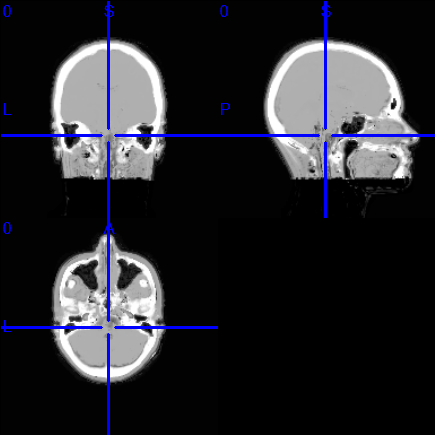
\includegraphics[width=\linewidth]{sct0.png}
\caption{sct0.png}
\end{figure}

\begin{figure}
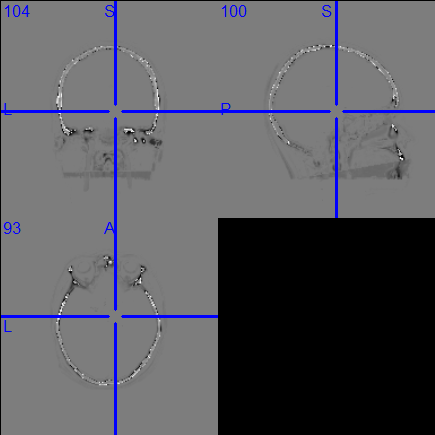
\includegraphics[width=\linewidth]{pdsct0.png}
\caption{Procent difference med værdier +- 100 sat til +- 100.}
\end{figure}

\begin{figure}
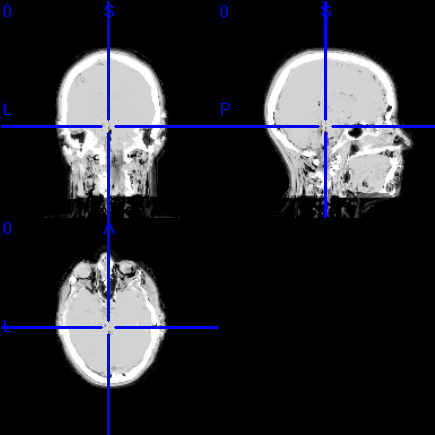
\includegraphics[width=\linewidth]{sct1.png}
\caption{sct1.png}
\end{figure}

\begin{figure}
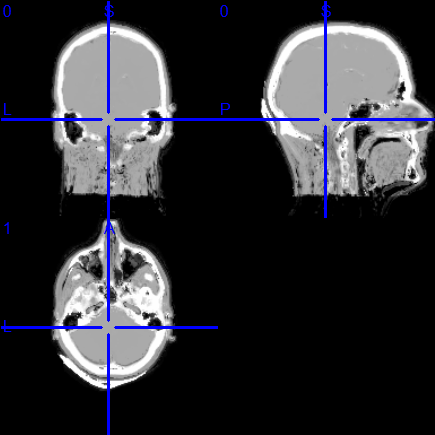
\includegraphics[width=\linewidth]{sct5.png}
\caption{sct5.png}
\end{figure}

\subsubsection{Udregn sCT til hjerner med artifakter trænet på hjerner uden artifakter}
\paragraph{Fremgangsmåde}
Træn på n hjerner test på m.

\paragraph{Forventning}

\paragraph{Resultat}

\subsubsection{Udregn sCT til hjerner trænet på hjerner med artifakter}
\paragraph{Fremgangsmåde}
Iterativt træn på et antal hjerner og introducer hjerner med artifakter.
Sammenlign kvaliteten af sCT afhængigt af andelen af hjerner, som har
artifakter.

\paragraph{Forventning}
At sCT's kvalitet forværes for hver introduceret hjerne med artifakt.

\paragraph{Resultat}


\subsubsection{Over tid}
\paragraph{Fremgangsmåde}
Træn på gamle hjerner, test på ny hjerner. Og omvendt.

\paragraph{Forventning}
Forventningen er sCT af samme kvalitet, som dem ved LOOCV-forsøget.

\paragraph{Resultat}

\subsubsection{Test på en masse}
\paragraph{Fremgangsmåde}
Iterativt træn på n+1 hjerner

\paragraph{Forventning}
Forventning er at efter 7-8 hjerner giver det ikke rigtig nogen
kvalitetsforskel.

\paragraph{Resultat}